\documentclass[12pt, twoside]{article}
\usepackage[letterpaper, margin=1in, headsep=0.5in]{geometry}
\usepackage[english]{babel}
\usepackage[utf8]{inputenc}
\usepackage{amsmath}
\usepackage{amsfonts}
\usepackage{amssymb}
\usepackage{tikz}
\usepackage{yhmath}
%\usetikzlibrary{quotes, angles}

\usepackage{graphicx}
\usepackage{enumitem}
\usepackage{multicol}

\usepackage{fancyhdr}
\pagestyle{fancy}
\fancyhf{}
\renewcommand{\headrulewidth}{0pt} % disable the underline of the header

\fancyhead[RE]{\thepage}
\fancyhead[RO]{\thepage \\ Name: \hspace{3cm}}
\fancyhead[L]{BECA / Dr. Huson / 10th Grade Geometry\\* 29 January 2020}

\begin{document}
\subsubsection*{9.10 Dow Now: Sectors, secants, \& chords calculations}
 \begin{enumerate}

 \item Circle $O$ has a diameter $AB=10$, as shown.
    \begin{center}
    \begin{tikzpicture}[scale=.6]
      \draw (0,0) circle[radius=5];
      \draw [thick]
      (0:5) node[right] {$A$}--(180:5) node[left] {$B$};
      \draw [thick] (0,0)--(72:5) node[above right] {$C$};
      \fill (0,0) circle[radius=0.1] node[below]{$O$};
      %\draw (75:1.8) node[above] {$C$};
      %\draw (290:5) node[below] {$D$};
    \end{tikzpicture}
  \end{center}
  \begin{enumerate}
    \item Find the circumference of circle $O$. \vspace{2.5cm}
    \item Find the area of the semi-circle with diameter $\overline{AB}$. \vspace{2.5cm}
    \item Given $m\angle AOC=72^\circ$. Find the area of the sector $AOC$. \vspace{2.5cm}
    \item Find the perimeter of the sector $AOC$.
  \end{enumerate}

\newpage
\item Given circle $O$ with chords $\overline{AD}$ and $\overline{BE}$ intersecting at $C$, as shown in the diagram. Given $m \wideparen{AB}=70^\circ$, $m \wideparen{BD}=80^\circ$, and $m \wideparen{DE}=110^\circ$.
  \begin{multicols}{2}
   \raggedcolumns
   \begin{enumerate}
     \item Find the $m\angle BED$. \vspace{1.3cm}
     \item Find the $m\angle ACB$. \vspace{2cm}
     \item Given $AC=4$ and $BC=3$, find $AB$. \vspace{2cm}
     \item Given $CE=6$, find $CD$. \vspace{2cm}
   \end{enumerate}
   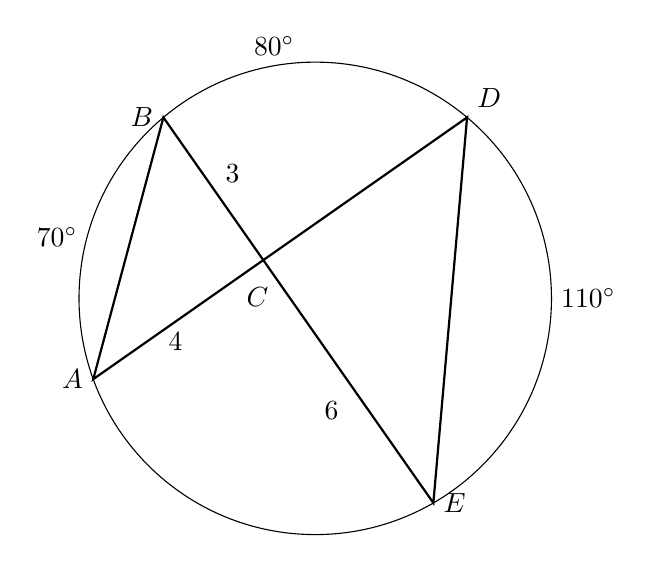
\begin{tikzpicture}[scale=.6]
     \draw (0,0) circle[radius=5];
     \draw [thick]
     (-60:5) node[right] {$E$}--
     (130:5) node[left] {$B$}--
     (200:5) node[left] {$A$}--
     (50:5) node[above right] {$D$}--cycle;
     \draw (160:1.3) node[below] {$C$};
     \draw (120:3.5) node[below] {$3$};
     \draw (190:3) node[below] {$4$};
     \draw (280:2.0) node[below] {$6$};
     \draw (0:5) node[right] {$110^\circ$};
     \draw (100:5) node[above] {$80^\circ$};
     \draw (165:5) node[left] {$70^\circ$};
   \end{tikzpicture}
  \end{multicols}
\vspace{2cm}

\item Given the circle $O$ with circumference $8\pi$.
  \begin{enumerate}
    \item Write down the formula for the circumference of a circle and solve for the radius yielding a circumference of $8\pi$. \vspace{1cm}
    \item Find the area of the circle.
  \end{enumerate}
  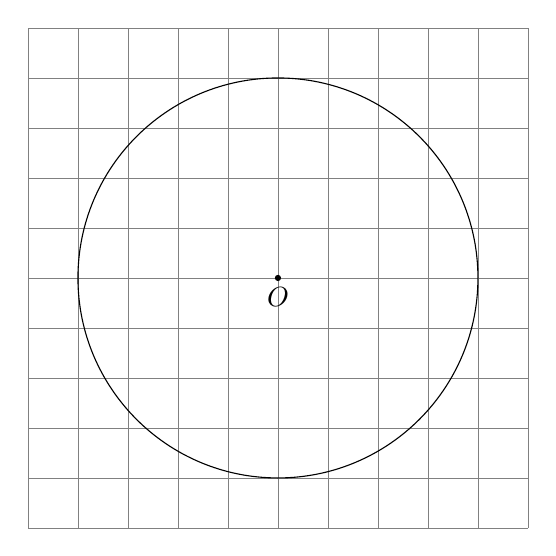
\begin{tikzpicture}[scale=.635]
    \draw [help lines] (-5,-5) grid (5,5);
    %\draw [thick, ->] (-2.2,0) -- (10.4,0) node [below right] {$x$};
    %\draw [thick, ->] (0,-2.2)--(0,10.4) node [left] {$y$};
    \draw (0,0) circle [radius=4] node[below]{$O$};
    \draw [fill] (0,0) circle [radius=0.05];
  \end{tikzpicture}

\item Given $\overleftrightarrow{RS}$ as shown on the number line, with $R=-3.1$ and $S=3.9$. \\[20pt] % Midpoint
  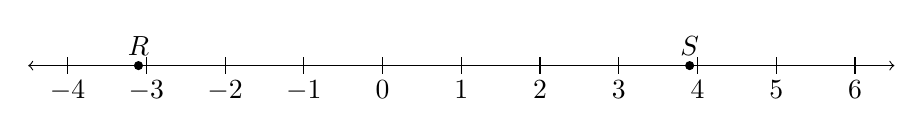
\begin{tikzpicture}
    \draw [<->] (-4.5,0)--(6.5,0);
    \foreach \x in {-4,...,6} %2 leading for diff!=1
      \draw[shift={(\x,0)},color=black] (0pt,-3pt) -- (0pt,3pt) node[below=5pt]  {$\x$};
      \draw [fill] (-3.1,0) circle [radius=0.05] node[above] {$R$};
      \draw [fill] (3.9,0) circle [radius=0.05] node[above] {$S$};
  \end{tikzpicture}
  \begin{enumerate}
    \item What is the exact distance on the number line between the points $R$ and $S$? \vspace{2cm} 
    \item The point $T$ bisects $\overline{RS}$. Find the value of $T$, and mark and label it on the numberline $\overleftrightarrow{RS}$ shown above. 
  \end{enumerate} \vspace{2cm} 

\newpage
\subsubsection*{9.10 Homework: Area and volume calculations}
\item In right triangle $ABC$ shown below, point $D$ is on $\overline{AB}$ and point $E$ is on $\overline{BC}$ such that $\overline{AC} \parallel \overline{DE}$. Given $BD=10$, $BC=12$, and $EC=4$.
  \begin{center}
    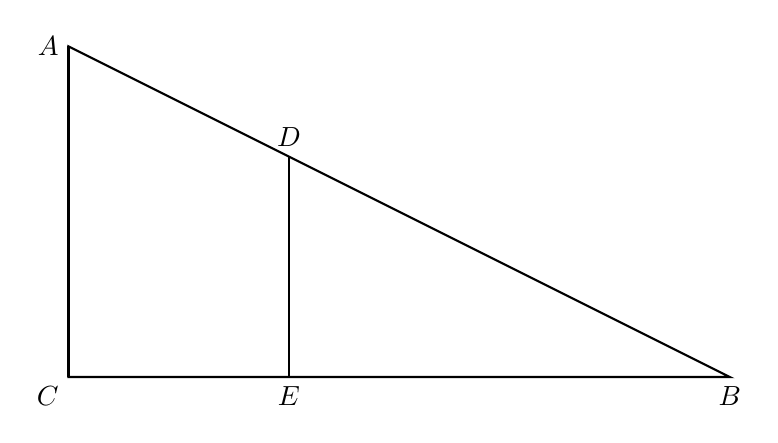
\begin{tikzpicture}[scale=0.7]
      \coordinate [label=left:$A$](A) at (-12,6);
      \coordinate [label=below:$B$](B) at (0, 0);
      \coordinate [label=below left:$C$](C) at (-12,0);
      \coordinate [label=above:$D$](D) at (-8, 4);
      \coordinate [label=below:$E$](E) at (-8,0);
      \draw [thick] (A)--(B)--(C)--cycle;
      \draw [thick] (A)--(C);
      \draw [thick] (D)--(E);
    \end{tikzpicture}
  \end{center}
\begin{enumerate}
  \item Find the length of $\overline{BE}$. \vspace{0.5cm}
  \item Find the scale factor, $k$, dilating $\triangle DBE \rightarrow \triangle ABC$, centered at $B$. \vspace{1.5cm}
  \item Find the area of $\triangle ABC$. \vspace{2.5cm}
  \item Find the area of $\triangle DEB$. \vspace{2.5cm}
  \item Find the ratio of the areas of the two triangles. \vspace{2.5cm}
  \end{enumerate}


\newpage
\item Find the area of a semi-circle radius of 7. \vspace{2cm}

\item Given circle $O$ with radius $OB=6$.
  \begin{multicols}{2}
   \raggedcolumns
   \begin{enumerate}
     \item Find the circumference of circle $O$. \vspace{1.7cm}
     \item Find its area.  \vspace{2cm}
     \item Given that $m\angle AOB=60^\circ$, find $m \wideparen{AB}$. \vspace{1cm}%yhmath package
     \item Find the area of the sector $AOB$. \vspace{1.5cm}
   \end{enumerate}
     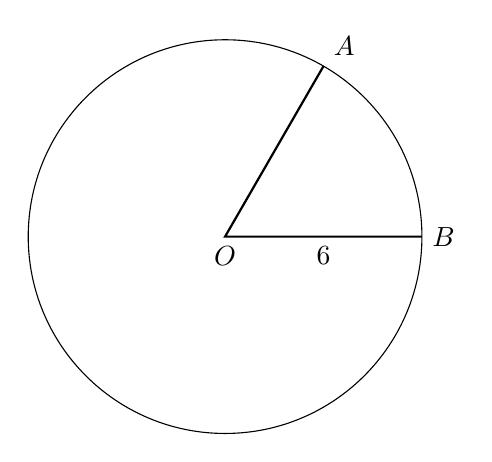
\begin{tikzpicture}[scale=.5]
       \draw (0,0) circle[radius=5];
       \draw [thick]
       (0:5) node[right] {$B$}--
       (0,0) node[below] {$O$}--
       (60:5) node[above right] {$A$};
       \draw (2.5,0) node[below] {$6$};
     \end{tikzpicture}
  \end{multicols}  \vspace{3cm}

\item Given circle $P$ with $m \wideparen{AB}=130^\circ$.
  \begin{multicols}{2}
    \raggedcolumns
    \begin{enumerate}
      \item Write down the $m\angle APB$. \vspace{1.7cm}
      \item Find the $m\angle AQB$. \vspace{2cm}
    \end{enumerate}
      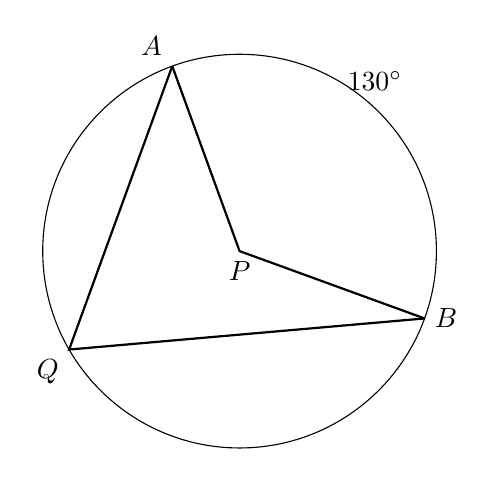
\begin{tikzpicture}[scale=.5]
        \draw (0,0) circle[radius=5];
        \draw [thick]
        (-20:5) node[right] {$B$}--
        (0,0) node[below] {$P$}--
        (110:5) node[above left] {$A$};
        \draw [thick] (-20:5)--(210:5) node[below left] {$Q$}--(110:5);
        \draw (60:5) node[right]{$130^\circ$};
      \end{tikzpicture}
  \end{multicols}

\newpage

\item Find the volume of a pyramid ($V=\frac{1}{3}Bh$) having a height of 11.3 inches and with a square base having side lengths of 7 inches. Express your result to the \emph{nearest cubic inch}. \vspace{5cm}

\item Find the volume of a hemisphere with a radius of 30 inches, to the \emph{nearest whole cubic inch}. (The formula for the volume of a \emph{sphere} is $V=\frac{4}{3}\pi r^3$)  \vspace{5cm}

\item Given $R(-2,0)$ and $S(3,5)$, find the length of $\overline{RS}$. Simplify the radical.

\newpage
\subsubsection*{9.8 Classwork: Analytical Geometry Practice}
\item Given the circle $C$ with circumference $10\pi$.
   \begin{enumerate}
     \item Write down the formula for the circumference of a circle and solve for the radius yielding a circumference of $6\pi$. \vspace{1cm}
     \item Find the area of the circle.
   \end{enumerate}
   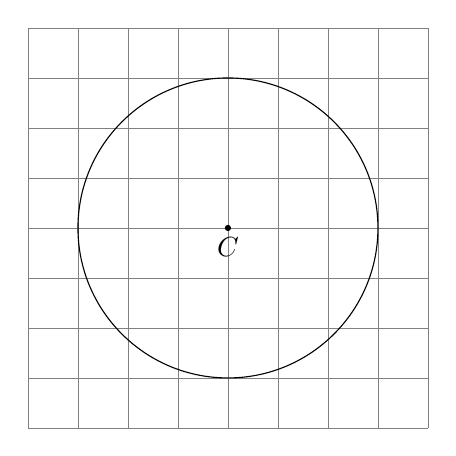
\begin{tikzpicture}[scale=.635]
     \draw [help lines] (-4,-4) grid (4,4);
     %\draw [thick, ->] (-2.2,0) -- (10.4,0) node [below right] {$x$};
     %\draw [thick, ->] (0,-2.2)--(0,10.4) node [left] {$y$};
     \draw (0,0) circle [radius=3] node[below]{$C$};
     \draw [fill] (0,0) circle [radius=0.05];
   \end{tikzpicture}

\newpage
\item In the diagram below, $\overline{AC}$ has endpoints with coordinates $A(-6,-3)$ and $C(6, 3)$.
  \begin{center} %4 quadrant regents grid
    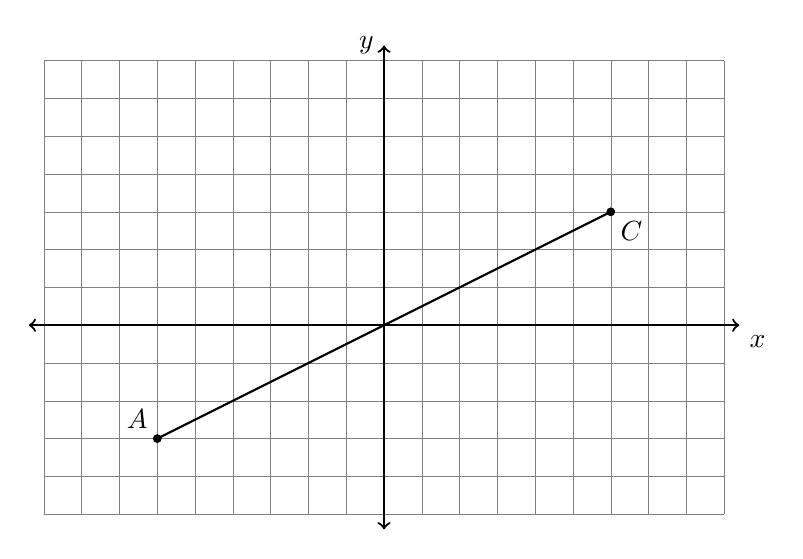
\begin{tikzpicture}[scale=.48]
      \draw [help lines] (-9,-5) grid (9,7);
      \draw [thick, <->] (-9.4,0) -- (9.4,0) node [below right] {$x$};
      \draw [thick, <->] (0,-5.4)--(0,7.4) node [left] {$y$};
      \draw [thick] (-6,-3)--(6, 3);
      \draw [fill] (-6,-3) circle [radius=0.1] node[above left] {$A$};
      \draw [fill] (6, 3) circle [radius=0.1] node[below right] {$C$};
    \end{tikzpicture}
  \end{center}
  If $B$ is a point on $\overline{AC}$ and $AB {:} BC = 1{:}3$,  what  are  the coordinates of $B$? \vspace{5cm}

\item Write down the center and radius of each circle.
  \begin{enumerate}
    \begin{multicols}{2}
    \item   $(x-4)^2+(y-3)^2=9$ \vspace{2.5cm}
    \item   $(x+5)^2+(y-2)^2=4^2$
    \item   $x^2+y^2=4$ \vspace{2.5cm}
    \item   $(x+7)^2+(y-2)^2=9^2$
    \end{multicols}
  \end{enumerate}

\newpage
\item Find the volume of a cone ($V=\frac{1}{3}\pi r^2 h$) having a height of 12 inches and with a radius of 3 inches. Express your result to the \emph{nearest cubic inch}. \vspace{5cm}

\item Find the volume of a cylinder 10 inches tall with a radius of 6 inches, to the \emph{nearest whole cubic inch}. (The formula for the volume of a \emph{cylinder} is $V=\frac{4}{3}\pi r^3$)  \vspace{5cm}

\item In  $\triangle ABC$ shown below, side $\overline{AC}$ is extended to point $D$ with $m\angle DAB=(6x-9)^\circ$, $m\angle C=35^\circ$, and $m\angle B=(4x+4)^\circ$.
  \begin{center}
    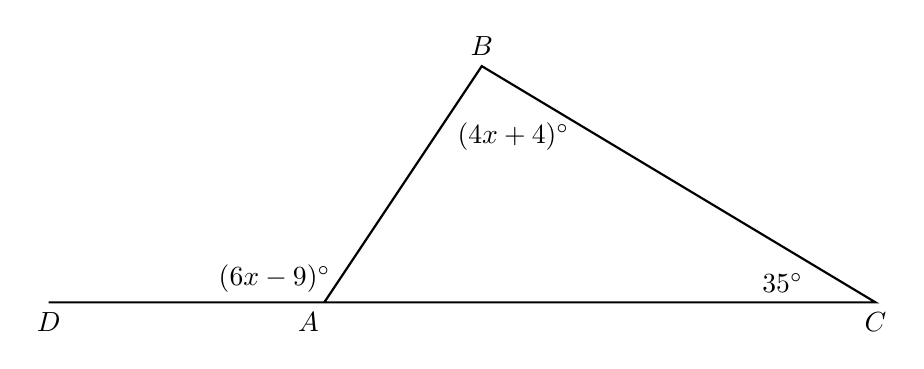
\begin{tikzpicture}
      \draw [thick](-1.5,0)node[below]{$D$}--
        (1.8,0)node[below]{$A$}--
        (9,0)node[below]{$C$}--
        (4,3)node[above]{$B$} --(2,0);
        \node at (2.2,0)[above left]{$(6x-9)^\circ$};
        \node at (8.2,0)[above left]{$35^\circ$};
        \node at (4.4,2.4)[below]{$(4x+4)^\circ$};
    \end{tikzpicture}
  \end{center}
  What is $m\angle BAC$?

\newpage
  \item On the set of axes below, graph the quadrilateral $ABCD$ having coordinates $A(-3,-3)$, $B(5,1)$, $C(6,8)$, and $D(-2,4)$.
    \begin{center} %4 quadrant regents grid
    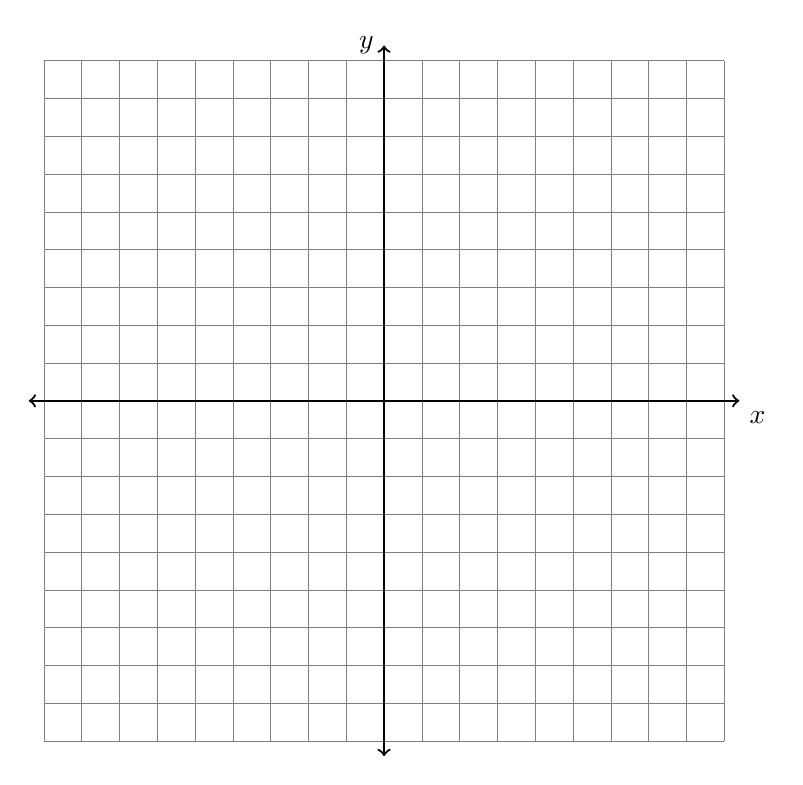
\begin{tikzpicture}[scale=.48]
      \draw [help lines] (-9,-9) grid (9,9);
      \draw [thick, <->] (-9.4,0) -- (9.4,0) node [below right] {$x$};
      \draw [thick, <->] (0,-9.4)--(0,9.4) node [left] {$y$};
      %\draw [thick] (-3,-3) node[below] {$A$}--
      %(5,1) node[right] {$B$}--
      %(6,8) node[left] {$C$}--
      %(-2,4) node[left] {$D$}--cycle;
      %\draw [fill] (5,0) circle [radius=0.1] node[above left] {$P$};
    \end{tikzpicture}
    \end{center}
    Show that the midpoints of the two diagonals, $\overline{AC}$ and $\overline{BD}$, are the same point. \\[5cm]
    Prove $ABCD$ is a parallelogram. Use the following theorem:
    A quadrilateral is a parallelogram if and only if its diagonals bisect each other. \\[0.5cm]
    Be sure to state the conclusion in your proof.

\newpage
\subsubsection*{9.8 Homework: Review Problem Set}
\item Given circle $O$ with chords $\overline{AD}$ and $\overline{BE}$ intersecting at $C$, as shown in the diagram. Given $m \wideparen{AB}=45^\circ$, $m \wideparen{BD}=108^\circ$, and $m \wideparen{DE}=65^\circ$.
  \begin{multicols}{2}
  \raggedcolumns
  \begin{enumerate}
    \item Find the $m\angle BAD$. \vspace{1.7cm}
    \item Find the $m\angle ACB$. \vspace{2cm}
  \end{enumerate}
  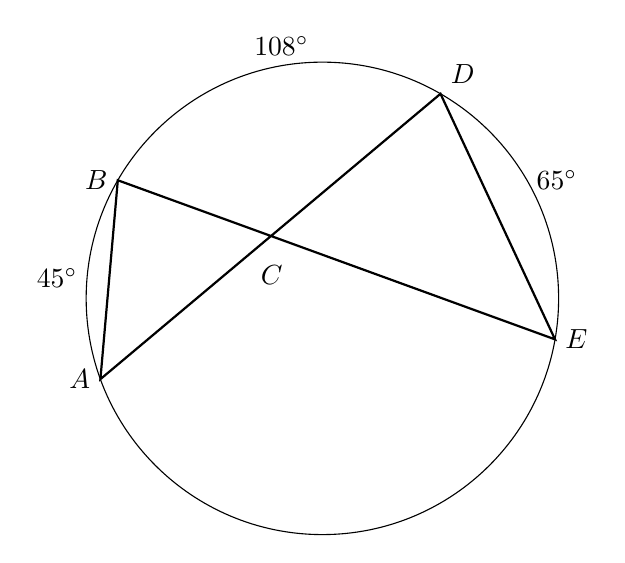
\begin{tikzpicture}[scale=.6]
    \draw (0,0) circle[radius=5];
    \draw [thick]
    (-10:5) node[right] {$E$}--
    (150:5) node[left] {$B$}--
    (200:5) node[left] {$A$}--
    (60:5) node[above right] {$D$}--cycle;
    \draw (140:1.4) node[below] {$C$};
    \draw (30:5) node[right] {$65^\circ$};
    \draw (100:5) node[above] {$108^\circ$};
    \draw (175:5) node[left] {$45^\circ$};
  \end{tikzpicture}
  \end{multicols}

\item On the graph, draw polygon ABCDEF with vertices A(1, 1), B(1, 4), C(3, 4), D(3, 7), E(8, 7), and F(8, 1). Find the perimeter and the area of the polygon.\\[1cm]
  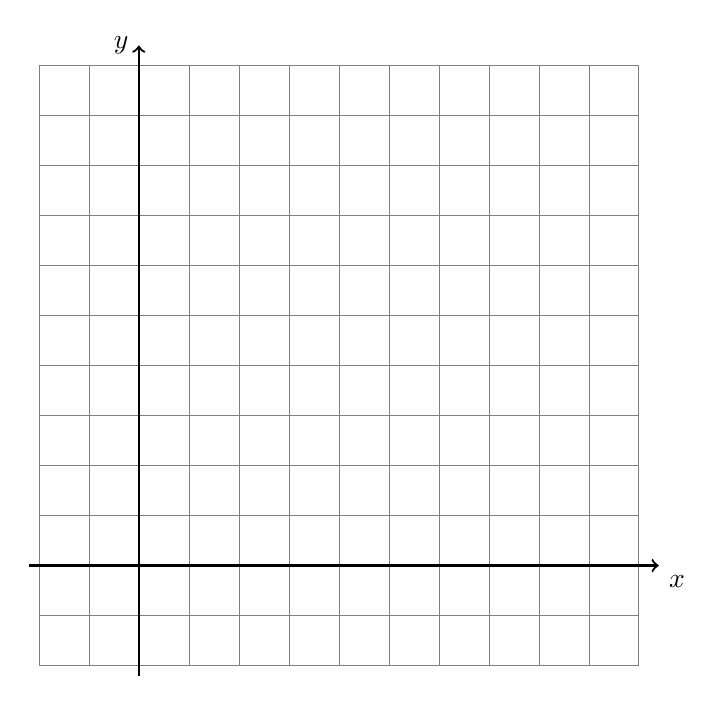
\begin{tikzpicture}[scale=.635]
    \draw [help lines] (-2,-2) grid (10,10);
    \draw [thick, ->] (-2.2,0) -- (10.4,0) node [below right] {$x$};
    \draw [thick, ->] (0,-2.2)--(0,10.4) node [left] {$y$};
  \end{tikzpicture}
  \vspace{2cm}

\newpage
\item Graph and label the two equations. Mark their intersection as an ordered pair.
  \begin{multicols}{2}
    $y = -4x-6$ \\
    $x-3y = -21$
  \end{multicols}  \vspace{1cm}
  Are the lines parallel, perpendicular, or neither? Justify your answer.
  \vspace{1.5cm}
  \begin{center} %4 quadrant regents grid w T-Chart
  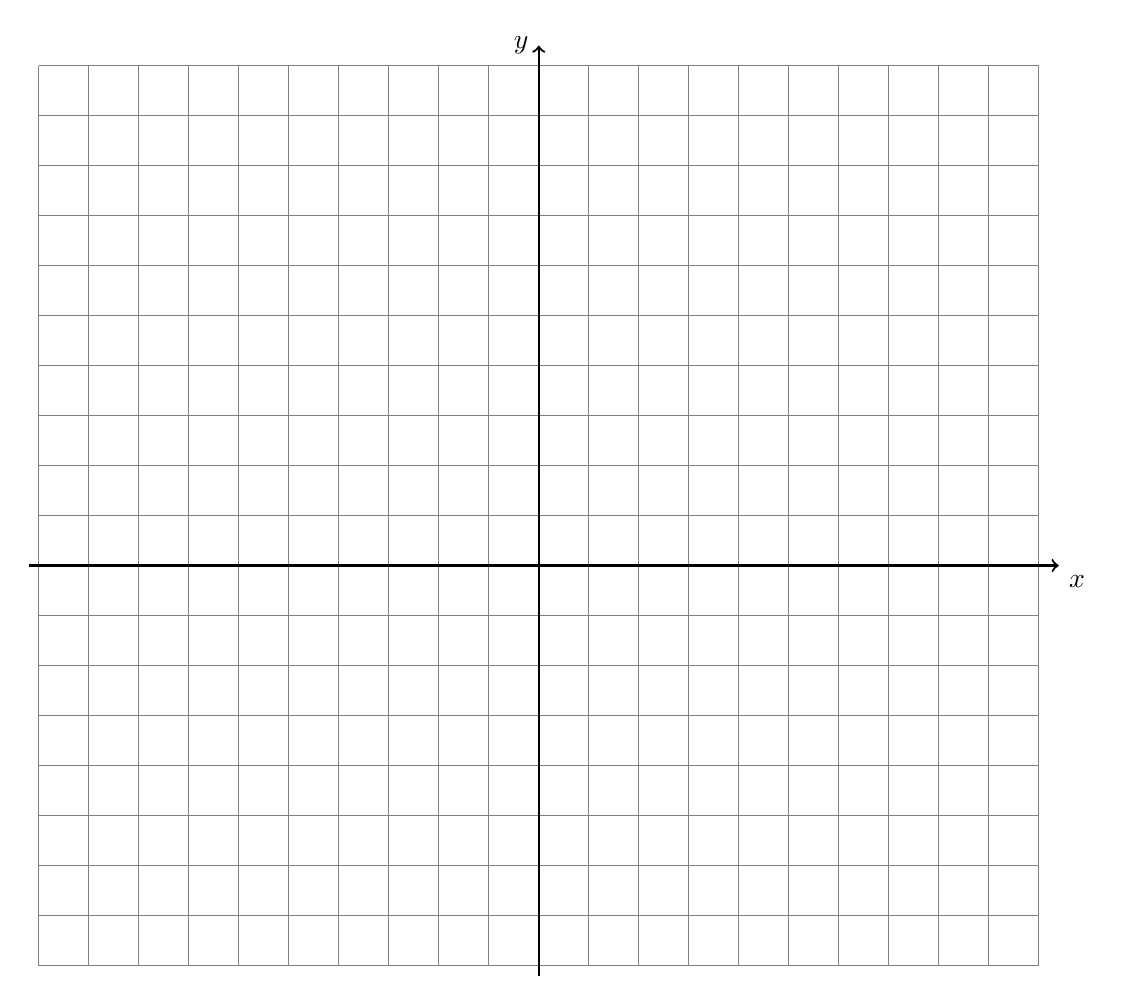
\begin{tikzpicture}[scale=.635]
    \draw [help lines] (-10,-8) grid (10,10);
    \draw [thick, ->] (-10.2,0) -- (10.4,0) node [below right] {$x$};
    \draw [thick, ->] (0,-8.2)--(0,10.4) node [left] {$y$};
  \end{tikzpicture}
  \end{center}

\item The line $l$ has the equation $y= 3x+2$.
  \begin{enumerate}
    \item What is the slope of the line $k$, given $k \parallel l$?
    \vspace{1cm}
    \item What is the slope of the line $m$, given $m \perp l$?
    \vspace{1cm}
  \end{enumerate}

\newpage
\item The secants $\overline{ABC}$ and $\overline{ADE}$ intersect the circle $O$, as shown in the diagram. \\Given $m \wideparen{BD}=28^\circ$ and $m \wideparen{CE}=136^\circ$.
  \begin{enumerate}
      \begin{multicols}{2}
        \item Find the $m\angle CDE$.
        \item Find the $m\angle BCD$.
      \end{multicols}  \vspace{1.5cm}
    \item Find the $m\angle A$. \vspace{0.5cm}
  \end{enumerate}
    \begin{center}
    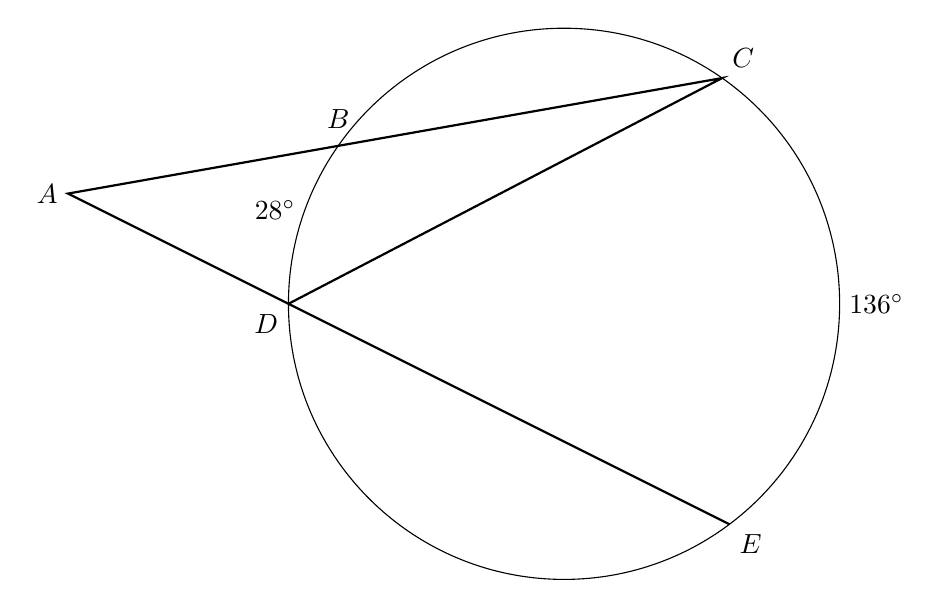
\begin{tikzpicture}[scale=.7]
      \draw (0,0) circle[radius=5];
      \draw [thick]
      (3,-4) node[below right] {$E$}--
      (-5,0) node[below left] {$D$}--
      (-9,2) node[left] {$A$}--
      (55:5) node[above right] {$C$}--
      (-5,0);
      \draw (138:5) node[left] {$B$};
      \draw (0:5) node[right] {$136^\circ$};
      \draw (160:5) node[left] {$28^\circ$};
    \end{tikzpicture}
  \end{center}

\item Express the result to the nearest thousandth.  \vspace{1cm}
  \begin{multicols}{2}
    \begin{enumerate}
      \item $\sin 35^\circ = $ \vspace{1cm}
      \item $\tan 70^\circ =$
      \item $\sin 78^\circ = $ \vspace{1cm}
      \item $\cos 12^\circ =$
    \end{enumerate}
  \end{multicols} \vspace{0.5cm}

\item Given $P(7,0)$ and $Q(3,2)$, find the length of $\overline{PQ}$. Simplify the radical.

\newpage
\item Given $m\angle R=45$ and $m\angle UST=110$. Find $m\angle U$.\\[1cm]
  \begin{tikzpicture}
    %\draw [->, thick] (0,0)--(5,5);
    \draw [<-, thick] (8,0)--(0,0)--(3,3)--(4.5,0);
    \draw [fill] (0,0) circle [radius=0.05] node[below]{$R$};
    \draw [fill] (4.5,0) circle [radius=0.05] node[below]{$S$};
    \draw [fill] (3,3) circle [radius=0.05] node[right]{$U$};
    \draw [fill] (7,0) circle [radius=0.05] node[below]{$T$};
  \end{tikzpicture}
  %\vspace{2cm}

\item On the graph below, draw $\overline{AB}$, with $A(5,3)$ and $B(-1,-3)$, labeling the end points. Determine and state the coordinates of the midpoint $M$ of $\overline{AB}$ and mark and label it on the graph.\\
  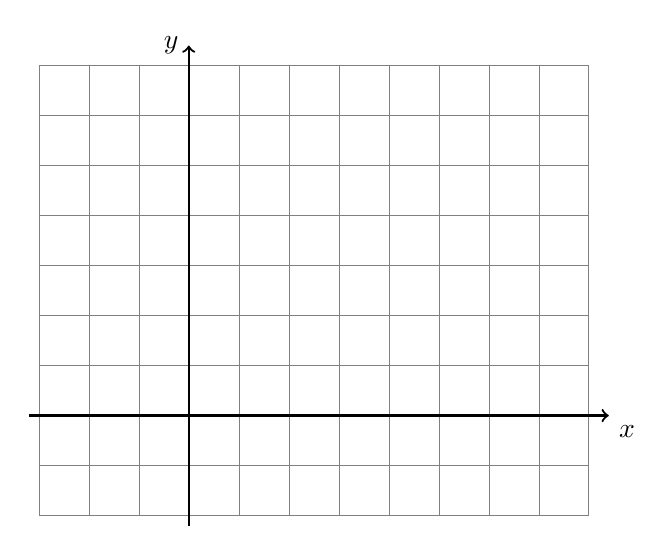
\begin{tikzpicture}[scale=.635]
    \draw [help lines] (-3,-2) grid (8,7);
    \draw [thick, ->] (-3.2,0) -- (8.4,0) node [below right] {$x$};
    \draw [thick, ->] (0,-2.2)--(0,7.4) node [left] {$y$};
  \end{tikzpicture}
  \vspace{0.5cm}

\item Given $\overline{ABC}$, $AC=18$, and the point $B$ partitions $\overline{AC}$ in a ratio of 2:7.\\[0.5cm] Find ${AB}$. \\[1.5cm]
    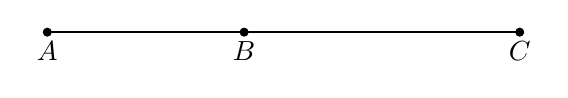
\begin{tikzpicture}
      \draw [-, thick] (1,0)--(7,0);
      \draw [fill] (1,0) circle [radius=0.05] node[below]{$A$};
      \draw [fill] (3.5,0) circle [radius=0.05] node[below]{$B$};
      \draw [fill] (7,0) circle [radius=0.05] node[below]{$C$};
    \end{tikzpicture} \vspace{3cm}

\end{enumerate}
\end{document}